\documentclass[12pt,english]{article}
\usepackage[T1]{fontenc}
\usepackage[latin9]{inputenc}
\usepackage{amsmath}
\usepackage{graphicx}

\makeatletter
\usepackage[letterpaper,body={6.5in,9in}, head=34pt, foot=70pt]{geometry}
\usepackage{fancyhdr}

\pdfpagewidth 8.5in
\pdfpageheight 11in

\pagestyle{fancy}
\headheight 35pt

\rhead{Fall 2021}
\chead{}
\lhead{MATH 3700 Operations Research}
\renewcommand{\footrulewidth}{0.4pt}
\rfoot{\thepage}
\cfoot{}
\lfoot{Wentworth Institute of Technology}

\usepackage{multicol}

\makeatother

\usepackage{babel}
\begin{document}
\textbf{Homework Assignment 3}\vspace{0.4cm}

\textbf{Due: }Sunday, October 17, 2021 in GS.\vspace{0.6cm}

\textbf{Name: Sunny Lee\underline{\hspace{12cm}}\vspace{0.4cm}}

\begin{enumerate}
    \item After running the dual-simplex algorithm, we get 625 as the optimal solution
    after 1 iteration. \\
    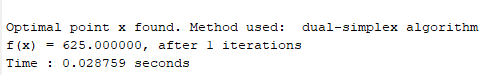
\includegraphics{1a.png}
    \item Comparing the dual-simplex and IPM, we find that although IPM had more iterations, 
    it took less time for IPM to converge on the optimal solution. \\
    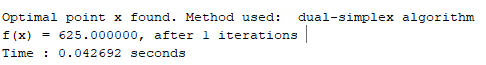
\includegraphics{2a.png}\\
    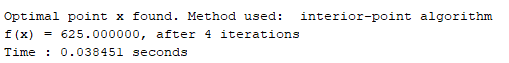
\includegraphics{2b.png}
    \item 
    To efficiently modify the program for different values of $n$, we must find a 
    way to efficiently generate matrices and vectors which have the form of the Klee
    Minty problem. 
    \item 
    The dual-simplex method required 1 iteration and took $0.042692$ seconds while the 
    IPM required 4 iterations and took $0.038451$ seconds. 
    \item 
    \item 
    The simplex method crashes after we let $n>28$. It took 1 iteration and $ .198109$ 
    seconds for the dual-simplex algorithm to converge. 
    \item 
    The IPM took 11 iterations and $.115121$ seconds to converge. 
    \item 
    The optimal solution for any value of $n$ is $5^n$. 
    \item 
    From the iterations above, we find that although the dual simplex method requires 
    less iterations, the interior point method tends to the optimal solution faster. 
    We also find that although the dual-simplex method crashes for $n$ values greater
    than 28, the IPM can go up to a value of 36. 
    
\end{enumerate}

\end{document}